\documentclass{article}
\usepackage{import}
\usepackage{amsmath}
\usepackage{tabularray}
\usepackage{float}


\import{lib/latex/}{wgmlgz}
\patchcmd{\thebibliography}{\section*}{\section}{}{}

\begin{document}
\itmo[
      variant=13,
      labn=5,
      discipline=Вычислительная математика,
      group=P3212,
      student=Соколов Анатолий Владимирович,
      teacher=Наумова Надежда Александровна 
]
\lstset{language=rust}
\newgeometry{
  a4paper,
  top=20mm,
  right=10mm,
  bottom=20mm,
  left=30mm
}
\tableofcontents
\section{Задание}
      \subsection{Обязательное задание (до 80 баллов)}
            \subsubsection{Вычислительная реализация задачи:}
                  \begin{enumerate}
                        \item Выбрать из табл. 1 заданную по варианту таблицу $y = f(x)$ (таблица 1.1);
                        \item Построить таблицу конечных разностей для заданной таблицы. Таблицу отразить в отчете;
                        \item Вычислить значения функции для аргумента $X_1$ (см. табл. 1.1), используя первую или вторую интерполяционную формулу Ньютона. Обратить внимание какой конкретно формулой необходимо воспользоваться;
                        \item Вычислить значения функции для аргумента $X_2$ (см. табл. 1.1), используя первую или вторую интерполяционную формулу Гаусса. Обратить внимание какой конкретно формулой необходимо воспользоваться;
                        \item Подробные вычисления привести в отчете.
                  \end{enumerate}

            \subsubsection{Программная реализация задачи:}
            \begin{enumerate}
                  \item Исходные данные задаются тремя способами:
                  \item \begin{enumerate}
                        \item в виде набора данных (таблицы $x,y$), пользователь вводит значения с клавиатуры;
                        \item в виде сформированных в файле данных (подготовить не менее трех тестовых вариантов);
                        \item на основе выбранной функции, из тех, которые предлагает программа, например, $\sin x$. Пользователь выбирает уравнение, исследуемый интервал и количество точек на интервале (не менее двух функций).
                  \end{enumerate}
                  \item Сформировать и вывести таблицу конечных разностей;
                  \item Вычислить приближенное значение функции для заданного значения аргумента, введенного с клавиатуры, указанными методами (см. табл. 2). Сравнить полученные значения;
                  \item Построить графики заданной функции с отмеченными узлами интерполяции и интерполяционного многочлена Ньютона/Гаусса (разными цветами);
                  \item Программа должна быть протестирована на различных наборах данных, в том числе и некорректных.
                  \item Проанализировать результаты работы программы.
            \end{enumerate}
            
      \subsection{Необязательное задание (до 20 баллов)}
            \begin{enumerate}
                  \item Реализовать в программе вычисление значения функции для заданного значения аргумента, введенного с клавиатуры, используя схемы Стирлинга;
                  \item Реализовать в программе вычисление значения функции для заданного значения аргумента, введенного с клавиатуры, используя схемы Бесселя.
            \end{enumerate}
      
\subsection{Вариант}
      \subsubsection{Варианты задания для вычислительной реализации задачи:}
            \begin{table}[H]
                  \begin{tabular}{|l|l|l|l|}
                        \hline
                        x      & y      & $X_1$  & $X_2$  \\ \hline
                        1.1000 & 0.2234 &  & \\ \hline
                        1.2500 & 1.2438 &  & \\ \hline
                        1.4000 & 2.2644 & 1.168 & 1.463 \\ \hline
                        1.5500 & 3.2984 & & \\ \hline
                        1.7000 & 4.3222 & & \\ \hline
                        1.8500 & 5.3516 & & \\ \hline
                        2.0000 & 6.3867 & & \\ \hline
                  \end{tabular}
                  \caption{\small \sl {Таблица 1.1}} 
            \end{table}
      \subsubsection{Методы для реализации в программе:}
            \begin{enumerate}
                  \item Многочлен Лагранжа,
                  \item Многочлен Ньютона с разделенными разностями,
                  \item Многочлен Ньютона с конечными разностями,
                  \item Многочлен Гаусса.
            \end{enumerate}
            \begin{table}[H]
                  \begin{tabular}{|l|l|}
                        \hline
                        № варианта & метод \\ \hline
                        13 & 1,2,3 \\ \hline
                  \end{tabular}
                  \caption{\small \sl {Таблица 1.2}} 
            \end{table}
\subsection{Цель работы}
      Решить задачу интерполяции, найти значения функции при заданных значениях аргумента, отличных от узловых точек.



\section{Выполнение}
      
      \subsection{Вычислительная часть}

      Для выполнения задания, я начну с создания таблицы конечных разностей для данных значений \( x \) и \( y \). Затем рассчитаю значения функции для \( X_1 \) и \( X_2 \) с использованием соответствующих интерполяционных формул Ньютона и Гаусса.

            \subsubsection{Таблица заданных значений}
                  Исходные данные из таблицы 1.1:

                  \[
                  \begin{array}{|c|c|}
                  \hline
                  x & y \\
                  \hline
                  1.1000 & 0.2234 \\
                  1.2500 & 1.2438 \\
                  1.4000 & 2.2644 \\
                  1.5500 & 3.2984 \\
                  1.7000 & 4.3222 \\
                  1.8500 & 5.3516 \\
                  2.0000 & 6.3867 \\
                  \hline
                  \end{array}
                  \]

            \subsubsection{Таблица конечных разностей}
                  Используя значения \( y \), рассчитаем разности:
                  \\
                  1. Первая разность: \(\Delta y_i = y_{i+1} - y_i\) \\
                  2. Вторая разность: \(\Delta^2 y_i = \Delta y_{i+1} - \Delta y_i\) \\
                  3. Так далее до необходимого уровня разностей.
                  \\
                  Давайте рассмотрим подробный процесс расчёта таблицы конечных разностей для данных значений \(x\) и \(y\), как если бы это делалось вручную. Приведённые данные:

                  \[
                  \begin{array}{|c|c|}
                  \hline
                  x & y \\
                  \hline
                  1.1000 & 0.2234 \\
                  1.2500 & 1.2438 \\
                  1.4000 & 2.2644 \\
                  1.5500 & 3.2984 \\
                  1.7000 & 4.3222 \\
                  1.8500 & 5.3516 \\
                  2.0000 & 6.3867 \\
                  \hline
                  \end{array}
                  \]

                  \textbf{Шаг 1: Первая разность \(\Delta y\)}

                  Первая разность \(\Delta y_i\) вычисляется как разность между последовательными значениями \(y\):

                  \[
                  \Delta y_i = y_{i+1} - y_i
                  \]

                  Выполним расчёты:
                  \\
                  \(\Delta y_1 = 1.2438 - 0.2234 = 1.0204\) \\
                  \(\Delta y_2 = 2.2644 - 1.2438 = 1.0206\) \\
                  \(\Delta y_3 = 3.2984 - 2.2644 = 1.0340\) \\
                  \(\Delta y_4 = 4.3222 - 3.2984 = 1.0238\) \\
                  \(\Delta y_5 = 5.3516 - 4.3222 = 1.0294\) \\
                  \(\Delta y_6 = 6.3867 - 5.3516 = 1.0351\) \\

                  \textbf{Шаг 2: Вторая разность \(\Delta^2 y\)}

                  Вторая разность \(\Delta^2 y_i\) вычисляется как разность между последовательными первыми разностями:

                  \[
                  \Delta^2 y_i = \Delta y_{i+1} - \Delta y_i
                  \]

                  Выполним расчёты:
                  \\
                  \(\Delta^2 y_1 = 1.0206 - 1.0204 = 0.0002\) \\
                  \(\Delta^2 y_2 = 1.0340 - 1.0206 = 0.0134\) \\
                  \(\Delta^2 y_3 = 1.0238 - 1.0340 = -0.0102\) \\
                  \(\Delta^2 y_4 = 1.0294 - 1.0238 = 0.0056\) \\
                  \(\Delta^2 y_5 = 1.0351 - 1.0294 = 0.0057\) \\

                  \textbf{Шаг 3 и далее: Высшие разности}

                  Продолжаем вычисления для более высоких порядков разностей:
                  \\   
                  \(\Delta^3 y_1 = 0.0134 - 0.0002 = 0.0132\) \\
                  \(\Delta^3 y_2 = -0.0102 - 0.0134 = -0.0236\) \\
                  \(\Delta^3 y_3 = 0.0056 + 0.0102 = 0.0158\) \\
                  \(\Delta^3 y_4 = 0.0057 - 0.0056 = 0.0001\) \\

                  Продолжим до достижения нулевых значений или до выхода за пределы массива данных.
                  \\
                  \textbf{Таблица конечных разностей:}
 
                  \[
                  \begin{array}{|c|c|c|c|c|c|c|c|}
                  \hline
                  y & \Delta y & \Delta^2 y & \Delta^3 y & \Delta^4 y & \Delta^5 y & \Delta^6 y \\
                  \hline
                  0.2234 & 1.0204 & 0.0002 & 0.0132 & -0.0368 & 0.0762 & -0.1313 \\
                  1.2438 & 1.0206 & 0.0134 & -0.0236 & 0.0394 & -0.0551 & 0.0000 \\
                  2.2644 & 1.0340 & -0.0102 & 0.0158 & -0.0157 & 0.0000 & 0.0000 \\
                  3.2984 & 1.0238 & 0.0056 & 0.0001 & 0.0000 & 0.0000 & 0.0000 \\
                  4.3222 & 1.0294 & 0.0057 & 0.0000 & 0.0000 & 0.0000 & 0.0000 \\
                  5.3516 & 1.0351 & 0.0000 & 0.0000 & 0.0000 & 0.0000 & 0.0000 \\
                  6.3867 & 0.0000 & 0.0000 & 0.0000 & 0.0000 & 0.0000 & 0.0000 \\
                  \hline
                  \end{array}
                  \]
            \subsubsection{Интерполяция Ньютона для \( X_1 = 1.168 \)}
                  Интерполяция Ньютона для \( X_1 = 1.168 \): Здесь я применил первую интерполяционную формулу Ньютона. Эта формула основана на значениях в начале списка данных и подразумевает использование прогрессивных конечных разностей. Формула выглядит так:
                  $$
                  N_5(x) = y_5 + t\Delta y_4 + \frac{t(t+1)}{2!}\Delta^2 y_3 + \frac{t(t+1)(t+2)}{3!}\Delta^3 y_2 +
                  $$
                  $$\frac{t(t+1)(t+2)(t+3)}{4!}\Delta^4 y_1 + \frac{t(t+1)(t+2)(t+3)(t+4)}{5!}\Delta^5 y_0$$
                  где \( t = \frac{x - x_0}{h} \).
                  
                  Для расчета значения функции в точке $X_1$ используем интерполяционную формулу Ньютона, учитывая что $X_1$ ближе к началу интервала.
 
                  \[
                  \begin{aligned}
                  P(X_1) = & 0.2234 \\
                        & + 0.4533 \times 1.0204 \\
                        & + \frac{0.4533 \times (0.4533-1)}{2} \times 0.0002 \\
                        & + \frac{0.4533 \times (0.4533-1) \times (0.4533-2)}{6} \times 0.0132 \\
                        & + \frac{0.4533 \times (0.4533-1) \times (0.4533-2) \times (0.4533-3)}{24} \times -0.0368 \\
                        & + \frac{0.4533 \times (0.4533-1) \times (0.4533-2) \times (0.4533-3) \times (0.4533-4)}{120} \times 0.0762 \\
                        & + \frac{0.4533 \times (0.4533-1) \times (0.4533-2) \times (0.4533-3) \times (0.4533-4) \times (0.4533-5)}{720} \times -0.1313.
                  \end{aligned}
                  \]

            \subsubsection{Интерполяция Гаусса для \( X_2 = 1.463 \)}
            
                  Интерполяция Гаусса для \( X_2 = 1.463 \): Здесь я использовал подход Гаусса для точек, расположенных ближе к середине набора данных. Так как \( X_2 \) находится ближе к середине списка значений \( x \), я использовал первую интерполяционную формулу Гаусса, подходящую для вычисления значений в центре списка. Формула выглядит следующим образом:
                  $$P_3(x) = y_0 + t\Delta y_0 + \cfrac{t(t-1)}{2!}\Delta^2 y_1 + 
                  \cfrac{(t+1)t(t-1)}{3!}\Delta^3 y_1 + 
                  \cfrac{(t+1)t(t-1)(t-2)}{4!}\Delta^4 y_2 + $$
                  $$\cfrac{(t+2)(t+1)t(t-1)(t-2)}{5!}\Delta^5 y_2 + 
                  \cfrac{(t+2)(t+1)t(t-1)(t-2)(t-3)}{6!}\Delta^6 y_3 $$
                  где \( k \) — индекс элемента, ближайшего к \( x \), и \( t = \frac{x - x_k}{h} \).

                  Для расчета значения функции в точке \( X_2 \) используем интерполяционную формулу Гаусса, оптимизированную для значений в середине таблицы.

                  Для вычисления значения функции в точке \( X_2 = 1.463 \) с помощью интерполяционной формулы Гаусса, сначала определим индекс \( k \), который соответствует значению \( x \), наиболее близкому к \( X_2 \). Этот шаг важен для того, чтобы выбрать подходящий центр для интерполяции.

                  Исходя из списка значений \( x \):

                  \[
                  x = [1.1000, 1.2500, 1.4000, 1.5500, 1.7000, 1.8500, 2.0000]
                  \]

                  точка \( X_2 = 1.463 \) находится между \( x_2 = 1.4000 \) и \( x_3 = 1.5500 \). Следовательно, ближайший индекс \( k = 2 \) (считая с нуля).

                  Для интерполяционной формулы Гаусса \( t \) вычисляется по формуле:

                  \[
                  t = \frac{X_2 - x_k}{h}
                  \]

                  где \( h = 1.5500 - 1.4000 = 0.1500 \).

                  \[
                  t = \frac{1.463 - 1.4000}{0.1500} \approx 0.42
                  \]

                  Используем интерполяционную формулу Гаусса, которая учитывает разности, симметричные относительно выбранного индекса \( k \). Разложение выглядит следующим образом:

                  \[
                  P(X_2) = y_k + t \Delta y_k + \frac{t(t-1)}{2!} \Delta^2 y_{k-1} + \frac{t(t-1)(t+1)}{3!} \Delta^3 y_{k-1} + \ldots
                  \]


                  \[
                  \begin{aligned}
                  P(X_2) = & y_2 + t \Delta y_2 + \frac{t(t-1)}{2!} \Delta^2 y_1 + \frac{t(t-1)(t+1)}{3!} \Delta^3 y_1 \\
                        & + \frac{t(t-1)(t+1)(t-2)}{4!} \Delta^4 y_0 + \frac{t(t-1)(t+1)(t-2)(t+2)}{5!} \Delta^5 y_0 \\
                        & + \frac{t(t-1)(t+1)(t-2)(t+2)(t-3)}{6!} \Delta^6 y_0.
                  \end{aligned}
                  \]

                  Подставляя уже известные значения:
                  \\
                  \( y_2 = 2.2644 \) \\
                  \( \Delta y_2 = 1.0340 \) \\
                  \( \Delta^2 y_1 = -0.0102 \) \\
                  \( \Delta^3 y_1 = 0.0158 \) \\
                  \( \Delta^4 y_0 = -0.0368 \) \\
                  \( \Delta^5 y_0 = 0.0762 \) \\
                  \( \Delta^6 y_0 = -0.1313 \) \\

                  Формула расширяется до:

                  \[
                  \begin{aligned}
                  P(X_2) = & 2.2644 + 0.42 \cdot 1.0340 + \frac{0.42 \cdot (0.42-1)}{2} \cdot -0.0102 + \frac{0.42 \cdot (0.42-1) \cdot (0.42+1)}{6} \cdot 0.0158 \\
                        & + \frac{0.42 \cdot (0.42-1) \cdot (0.42+1) \cdot (0.42-2)}{24} \cdot -0.0368 \\
                        & + \frac{0.42 \cdot (0.42-1) \cdot (0.42+1) \cdot (0.42-2) \cdot (0.42+2)}{120} \cdot 0.0762 \\
                        & + \frac{0.42 \cdot (0.42-1) \cdot (0.42+1) \cdot (0.42-2) \cdot (0.42+2) \cdot (0.42-3)}{720} \cdot -0.1313.
                  \end{aligned}
                  \]
            \subsubsection{Результаты интерполяции}
                  
                  Значение функции в точке \( X_1 = 1.168 \), рассчитанное с использованием интерполяционной формулы Ньютона, составляет приблизительно \( 0.6934 \).
                  \\
                  Значение функции в точке \( X_2 = 1.463 \), рассчитанное с использованием интерполяционной формулы Гаусса, составляет \( 2.2644 \).
            
      \subsection{Блок-схема реализованного алгоритма}
            %  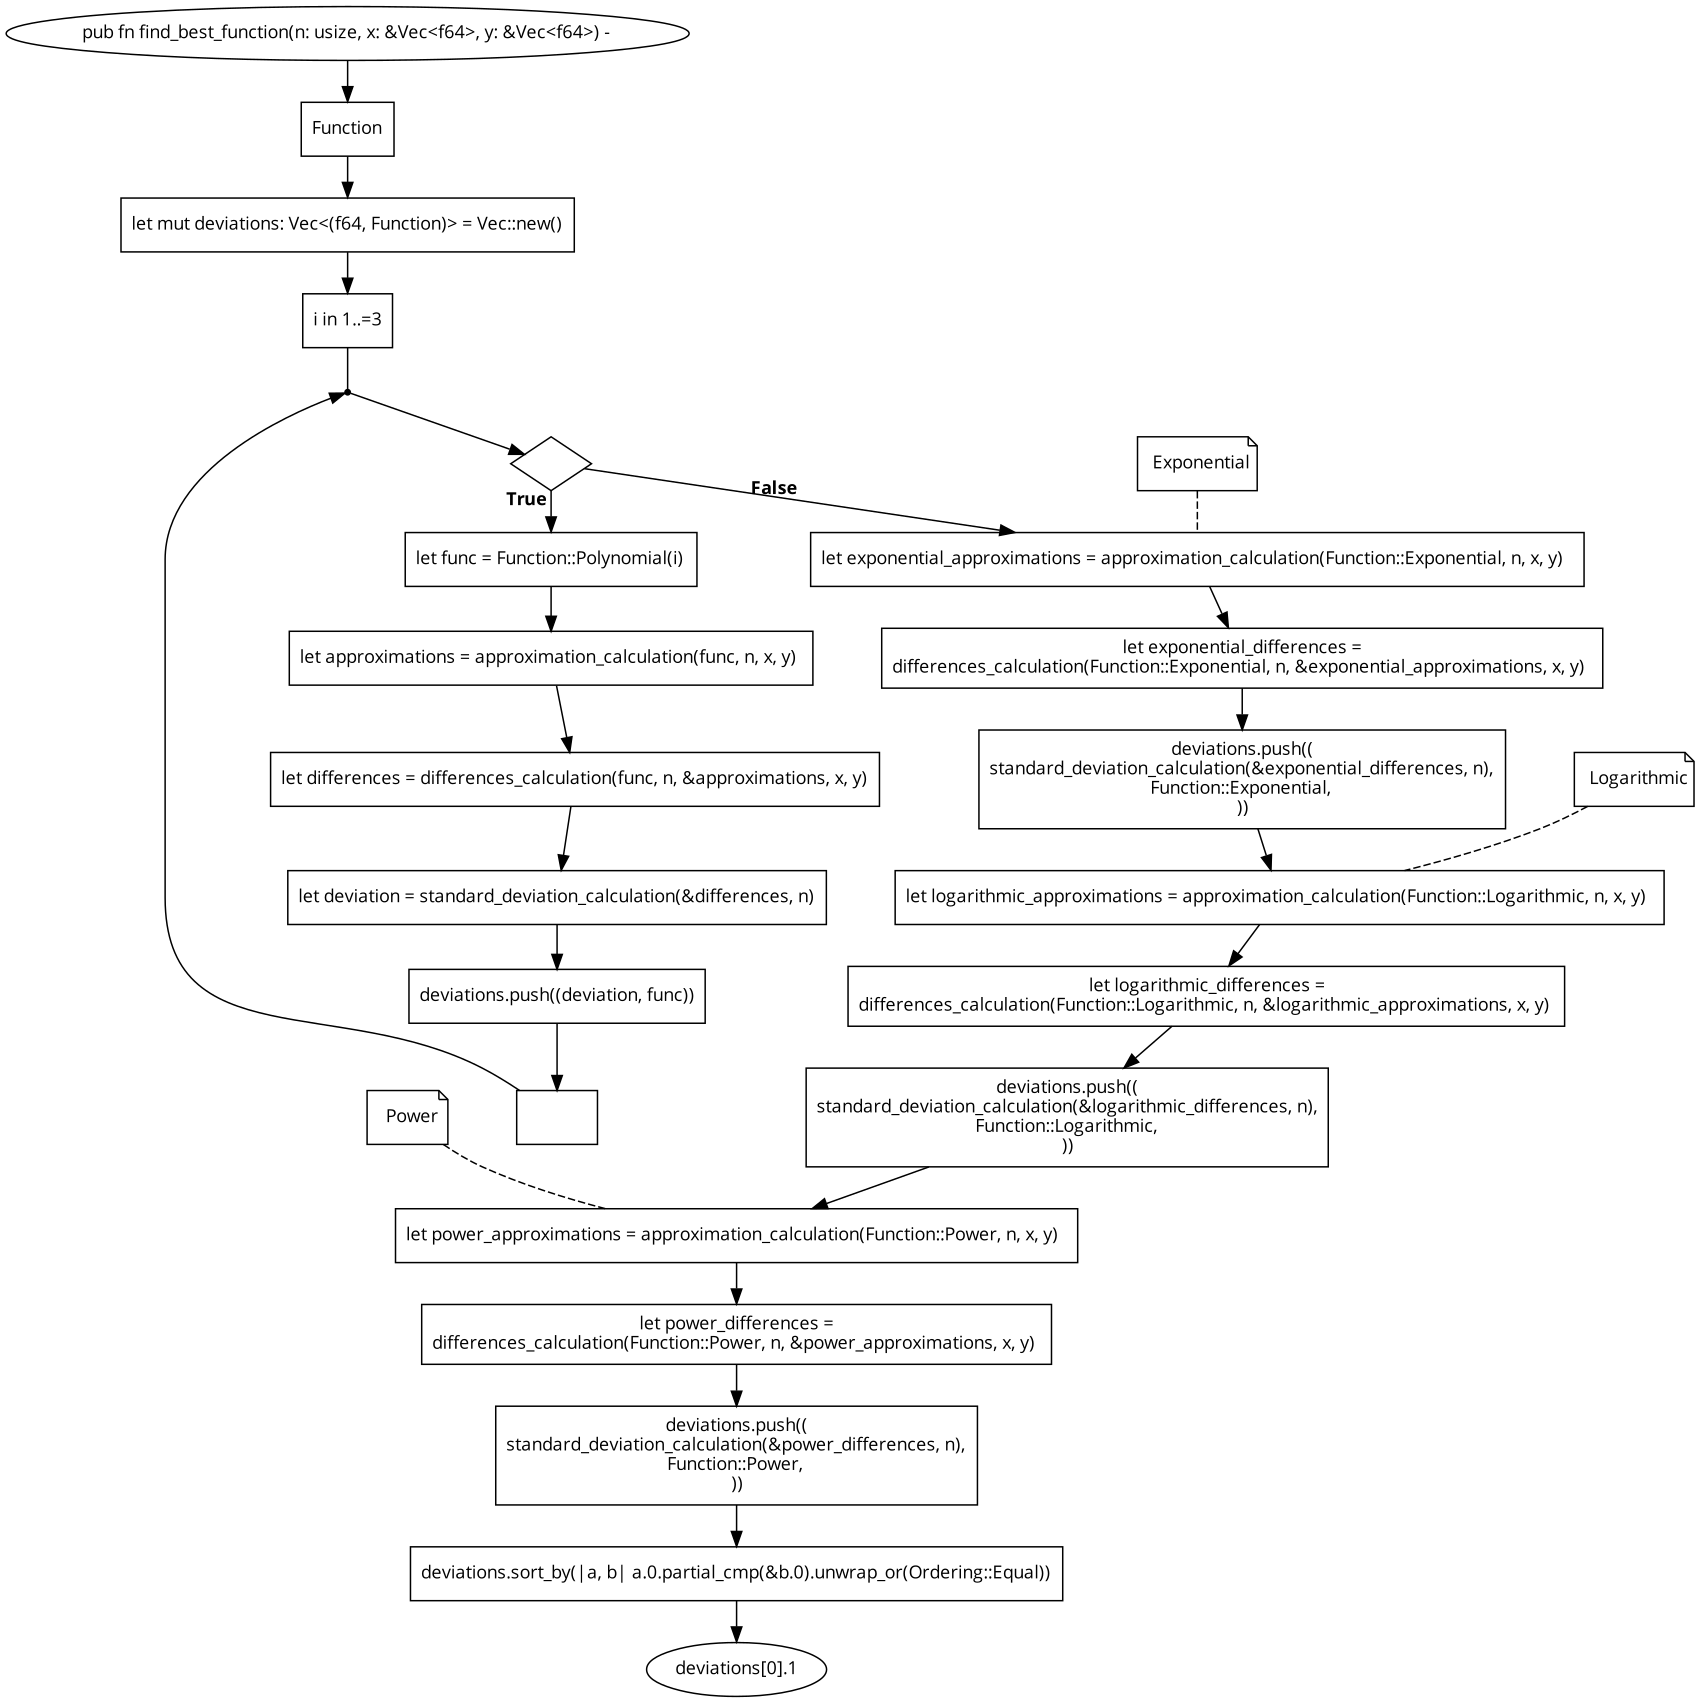
\includegraphics[scale=0.2]{best_function.png}
            %  \\
            %  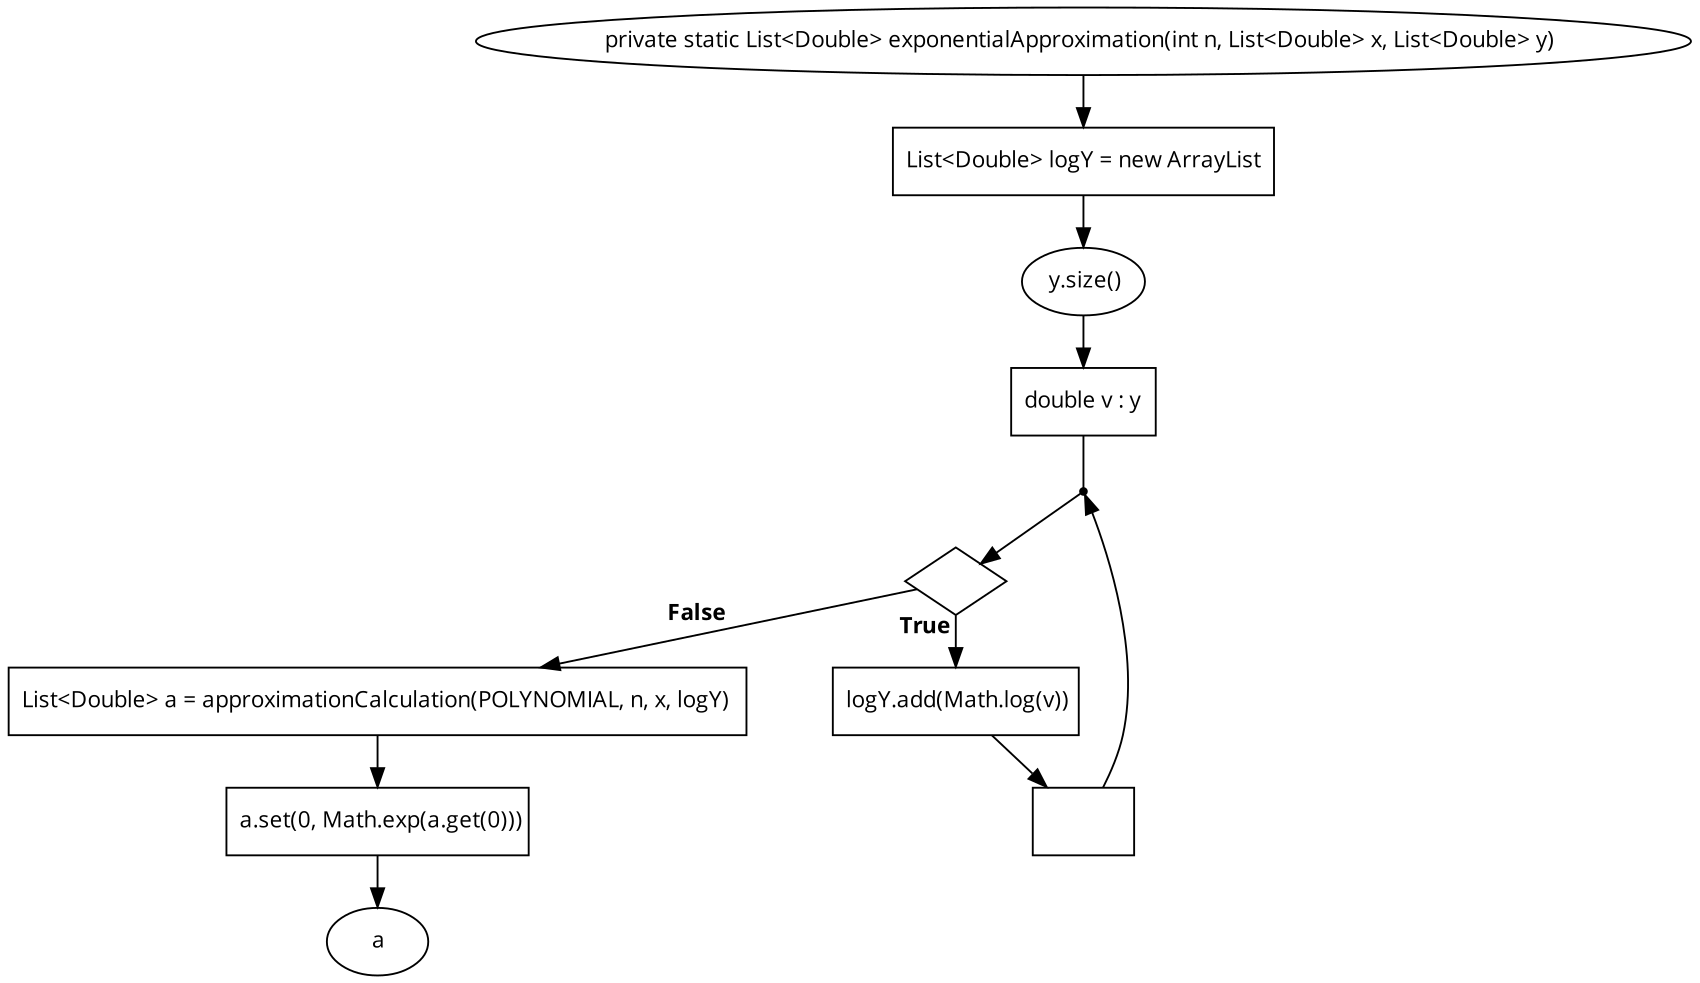
\includegraphics[scale=0.2]{exp_approx.png}
            %  \\
            %  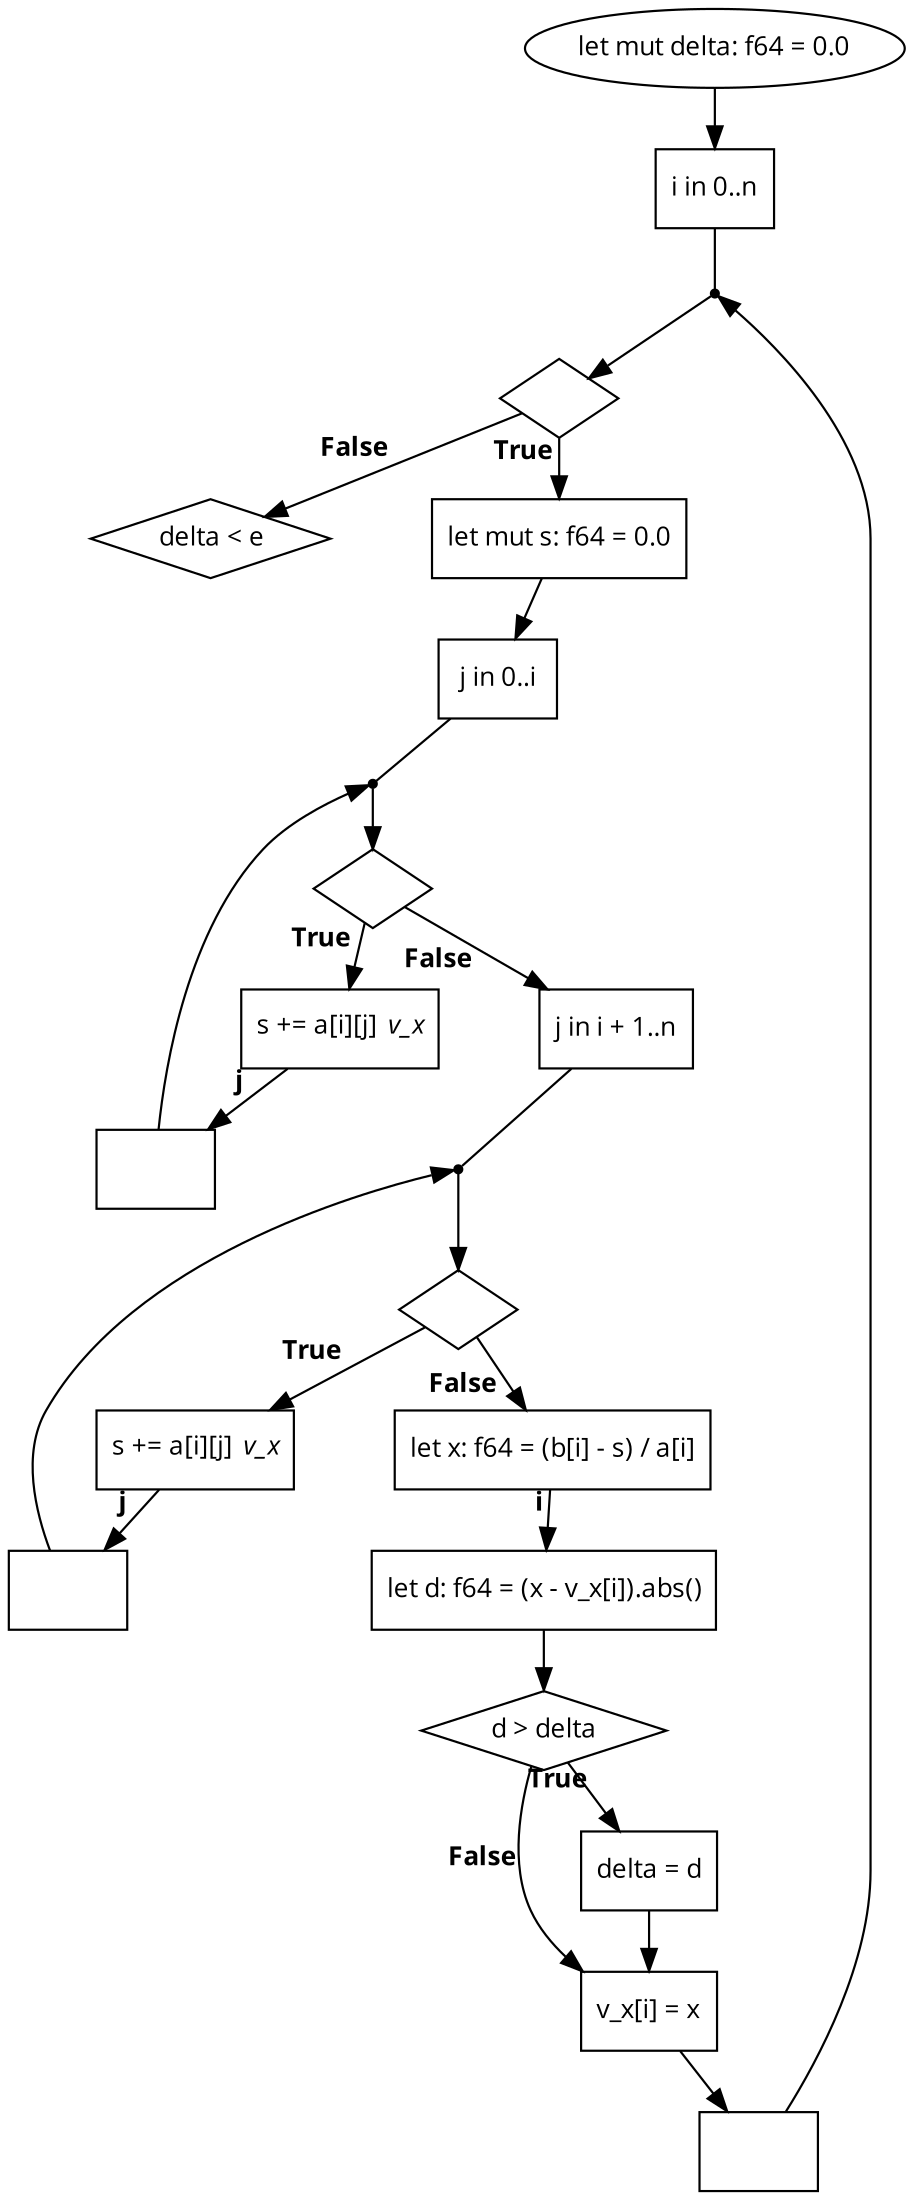
\includegraphics[scale=0.2]{lin_calc.png}
            %  \\
            %  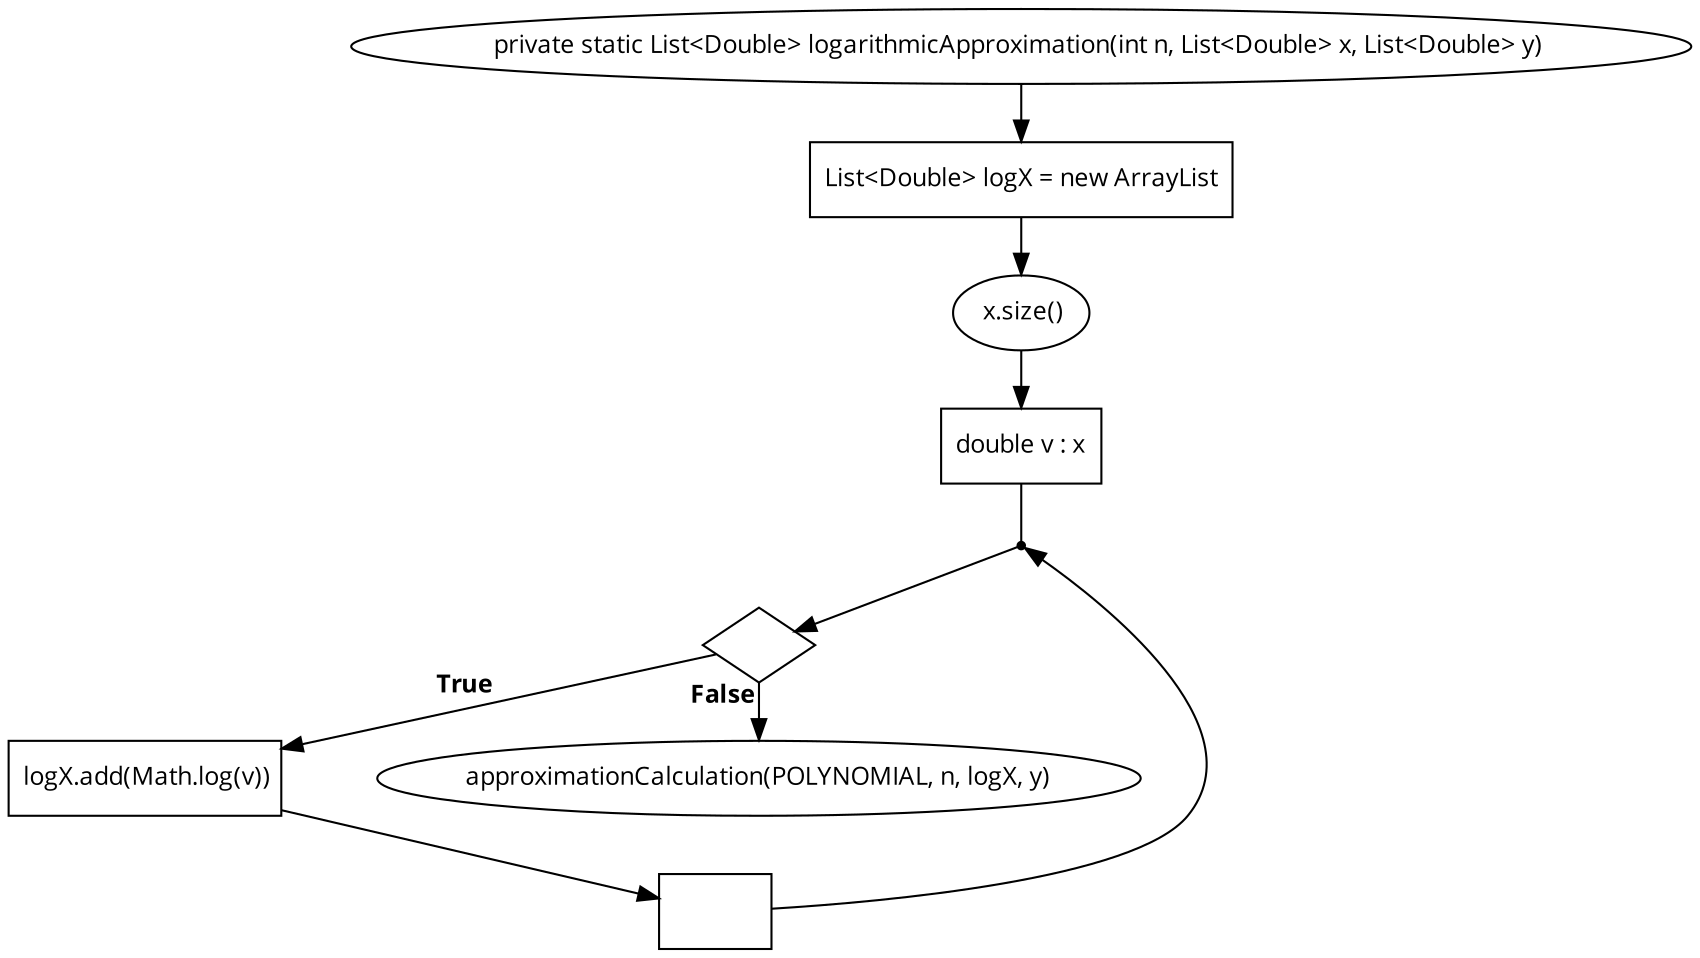
\includegraphics[scale=0.2]{log_approx.png}
            %  \\
            %  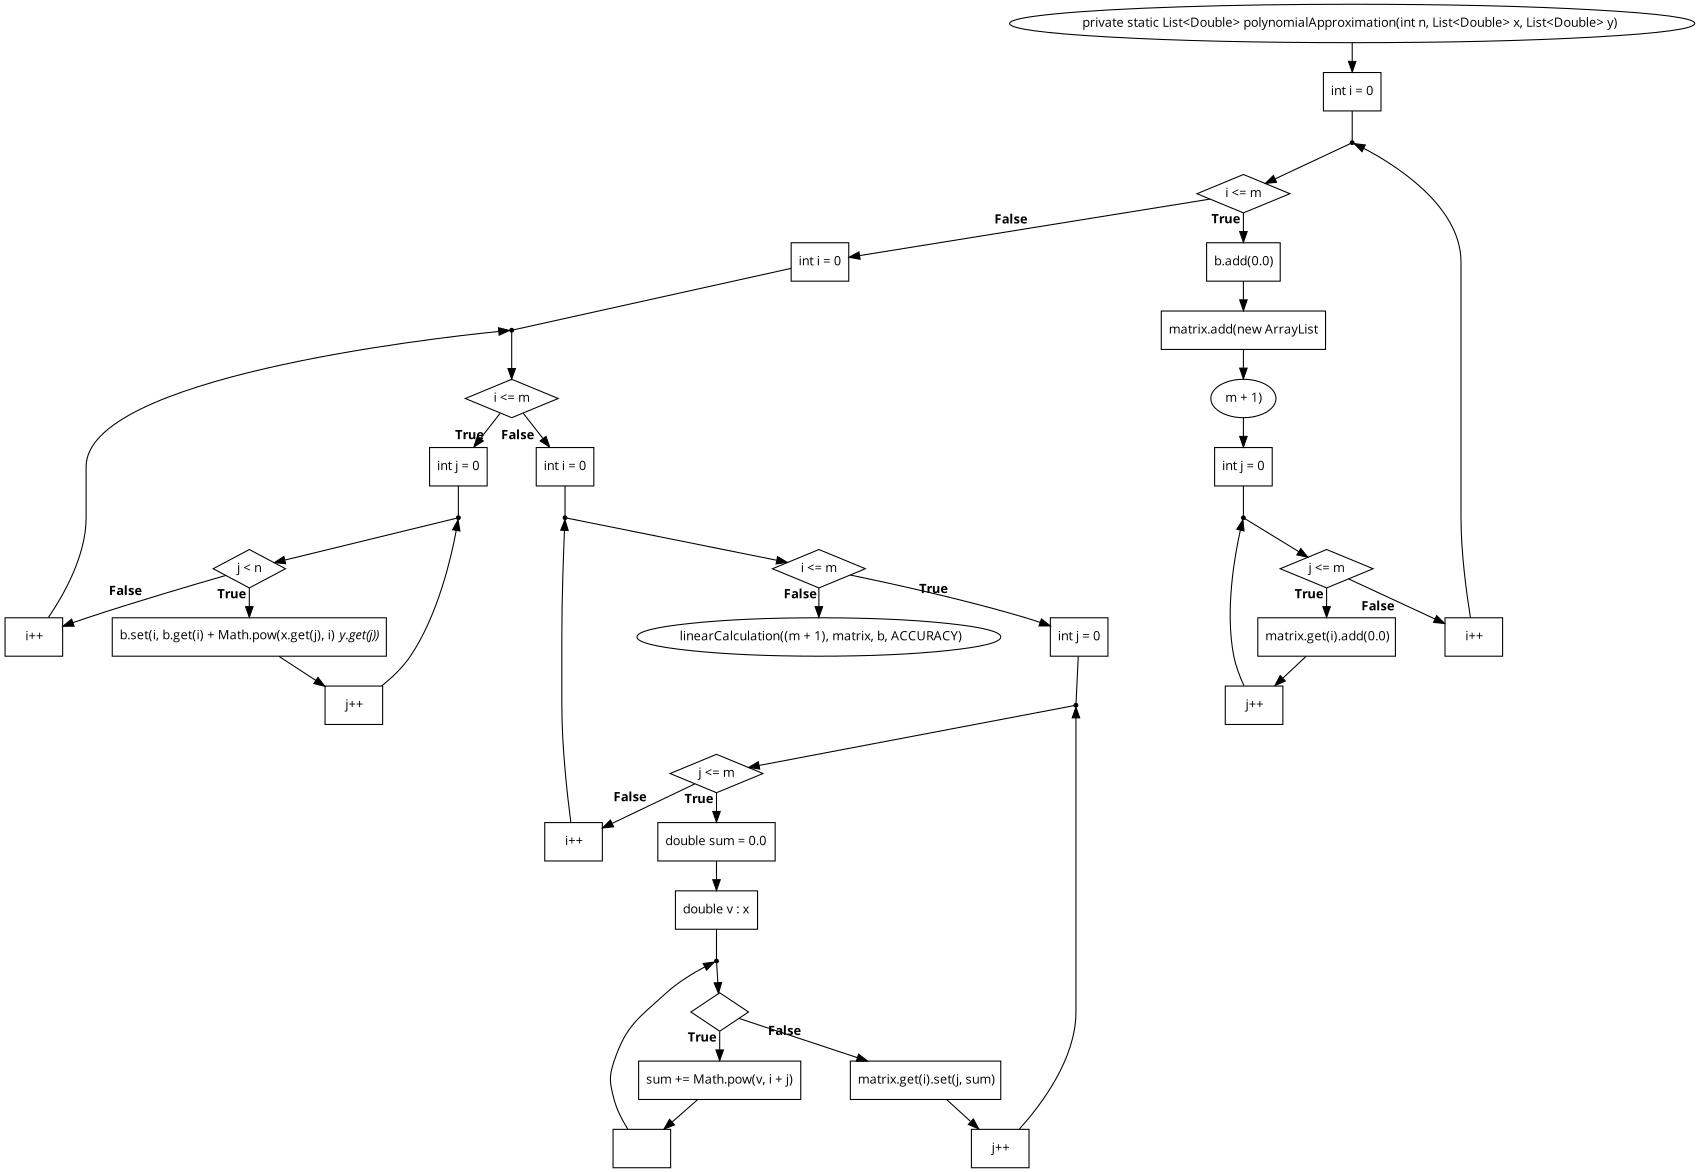
\includegraphics[scale=0.2]{polynom_approx.png}
            %  \\
            %  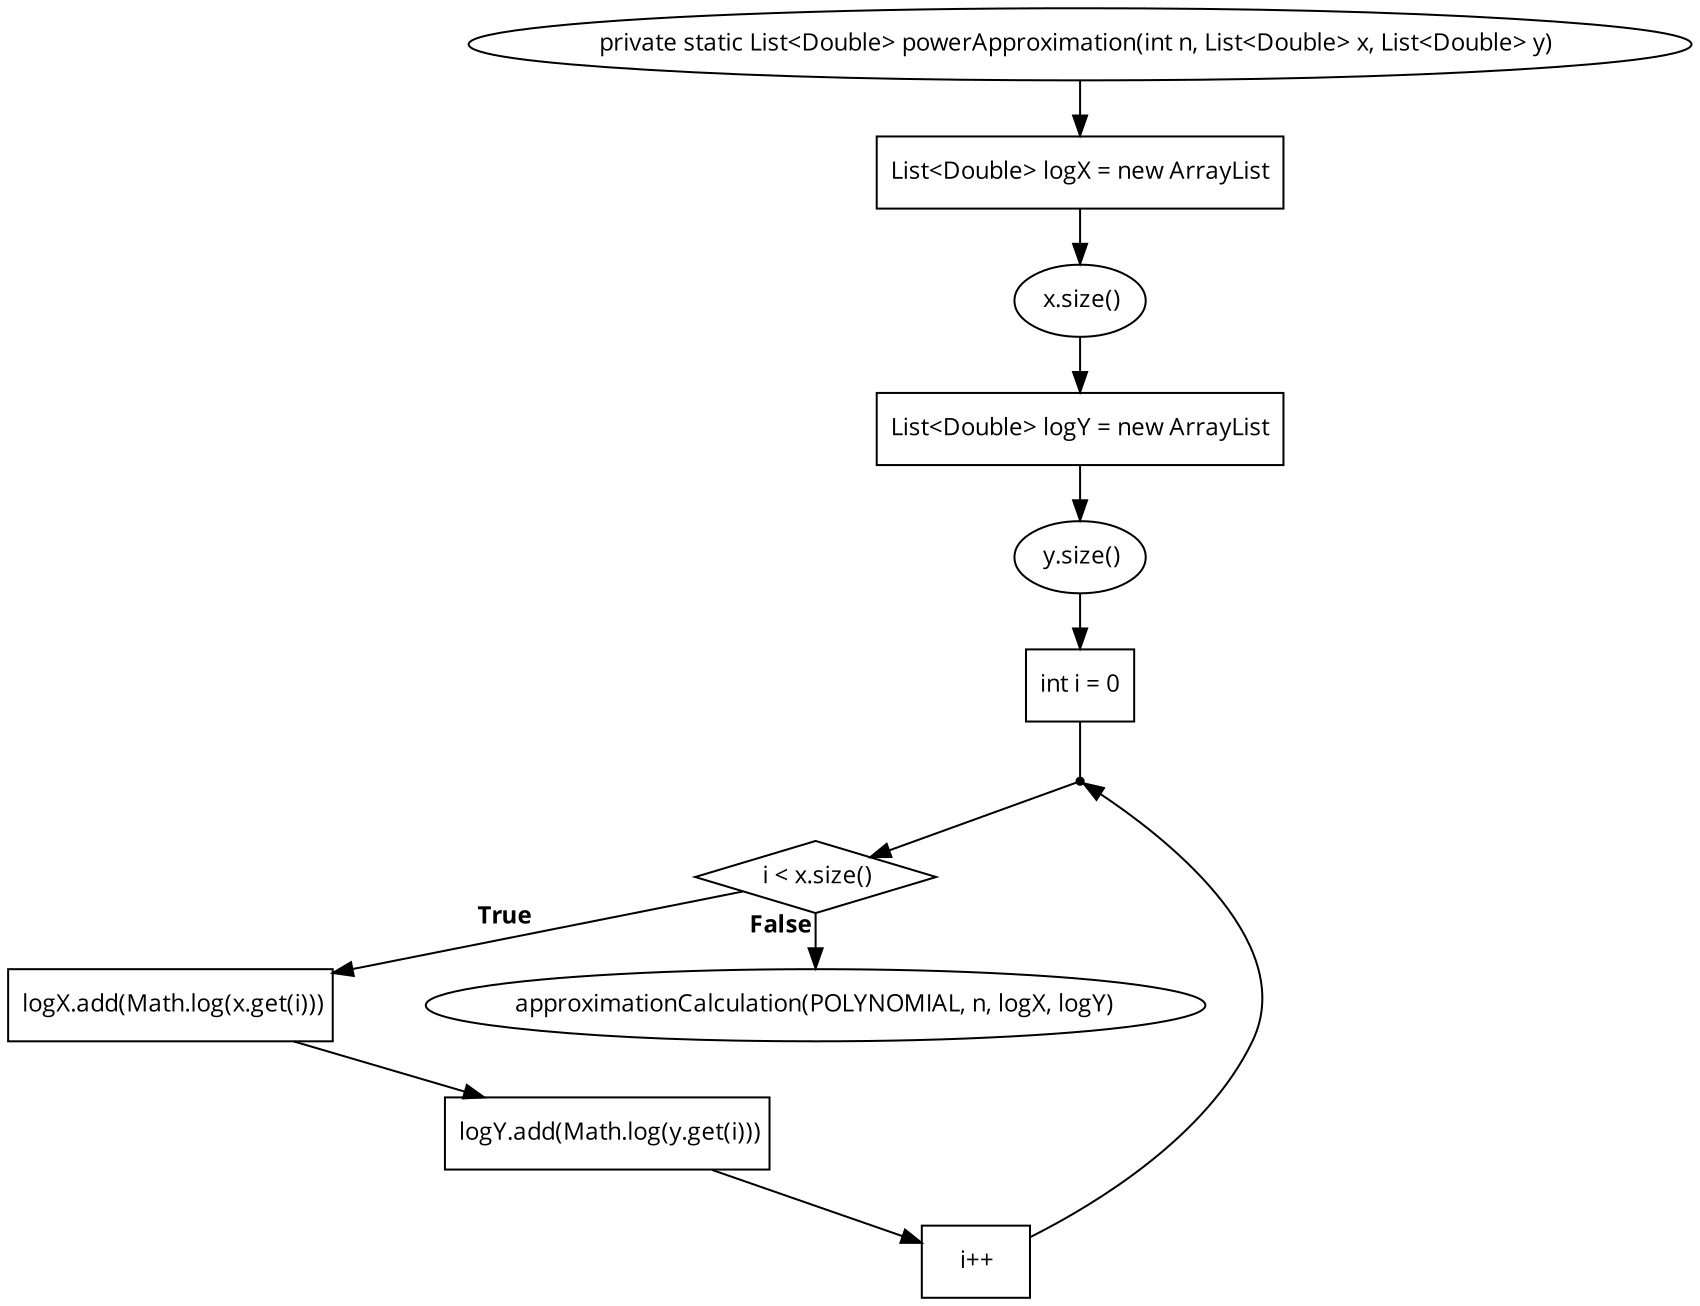
\includegraphics[scale=0.2]{power_approx.png}
             
      \subsection{Ссылка на GitHub c основной реализацией}
            \href{https://github.com/isofinly/compmath}{Github}

      \subsection{Примеры и результаты работы программы}
            \begin{figure}[H] 
                  \begin{center}  
                        %  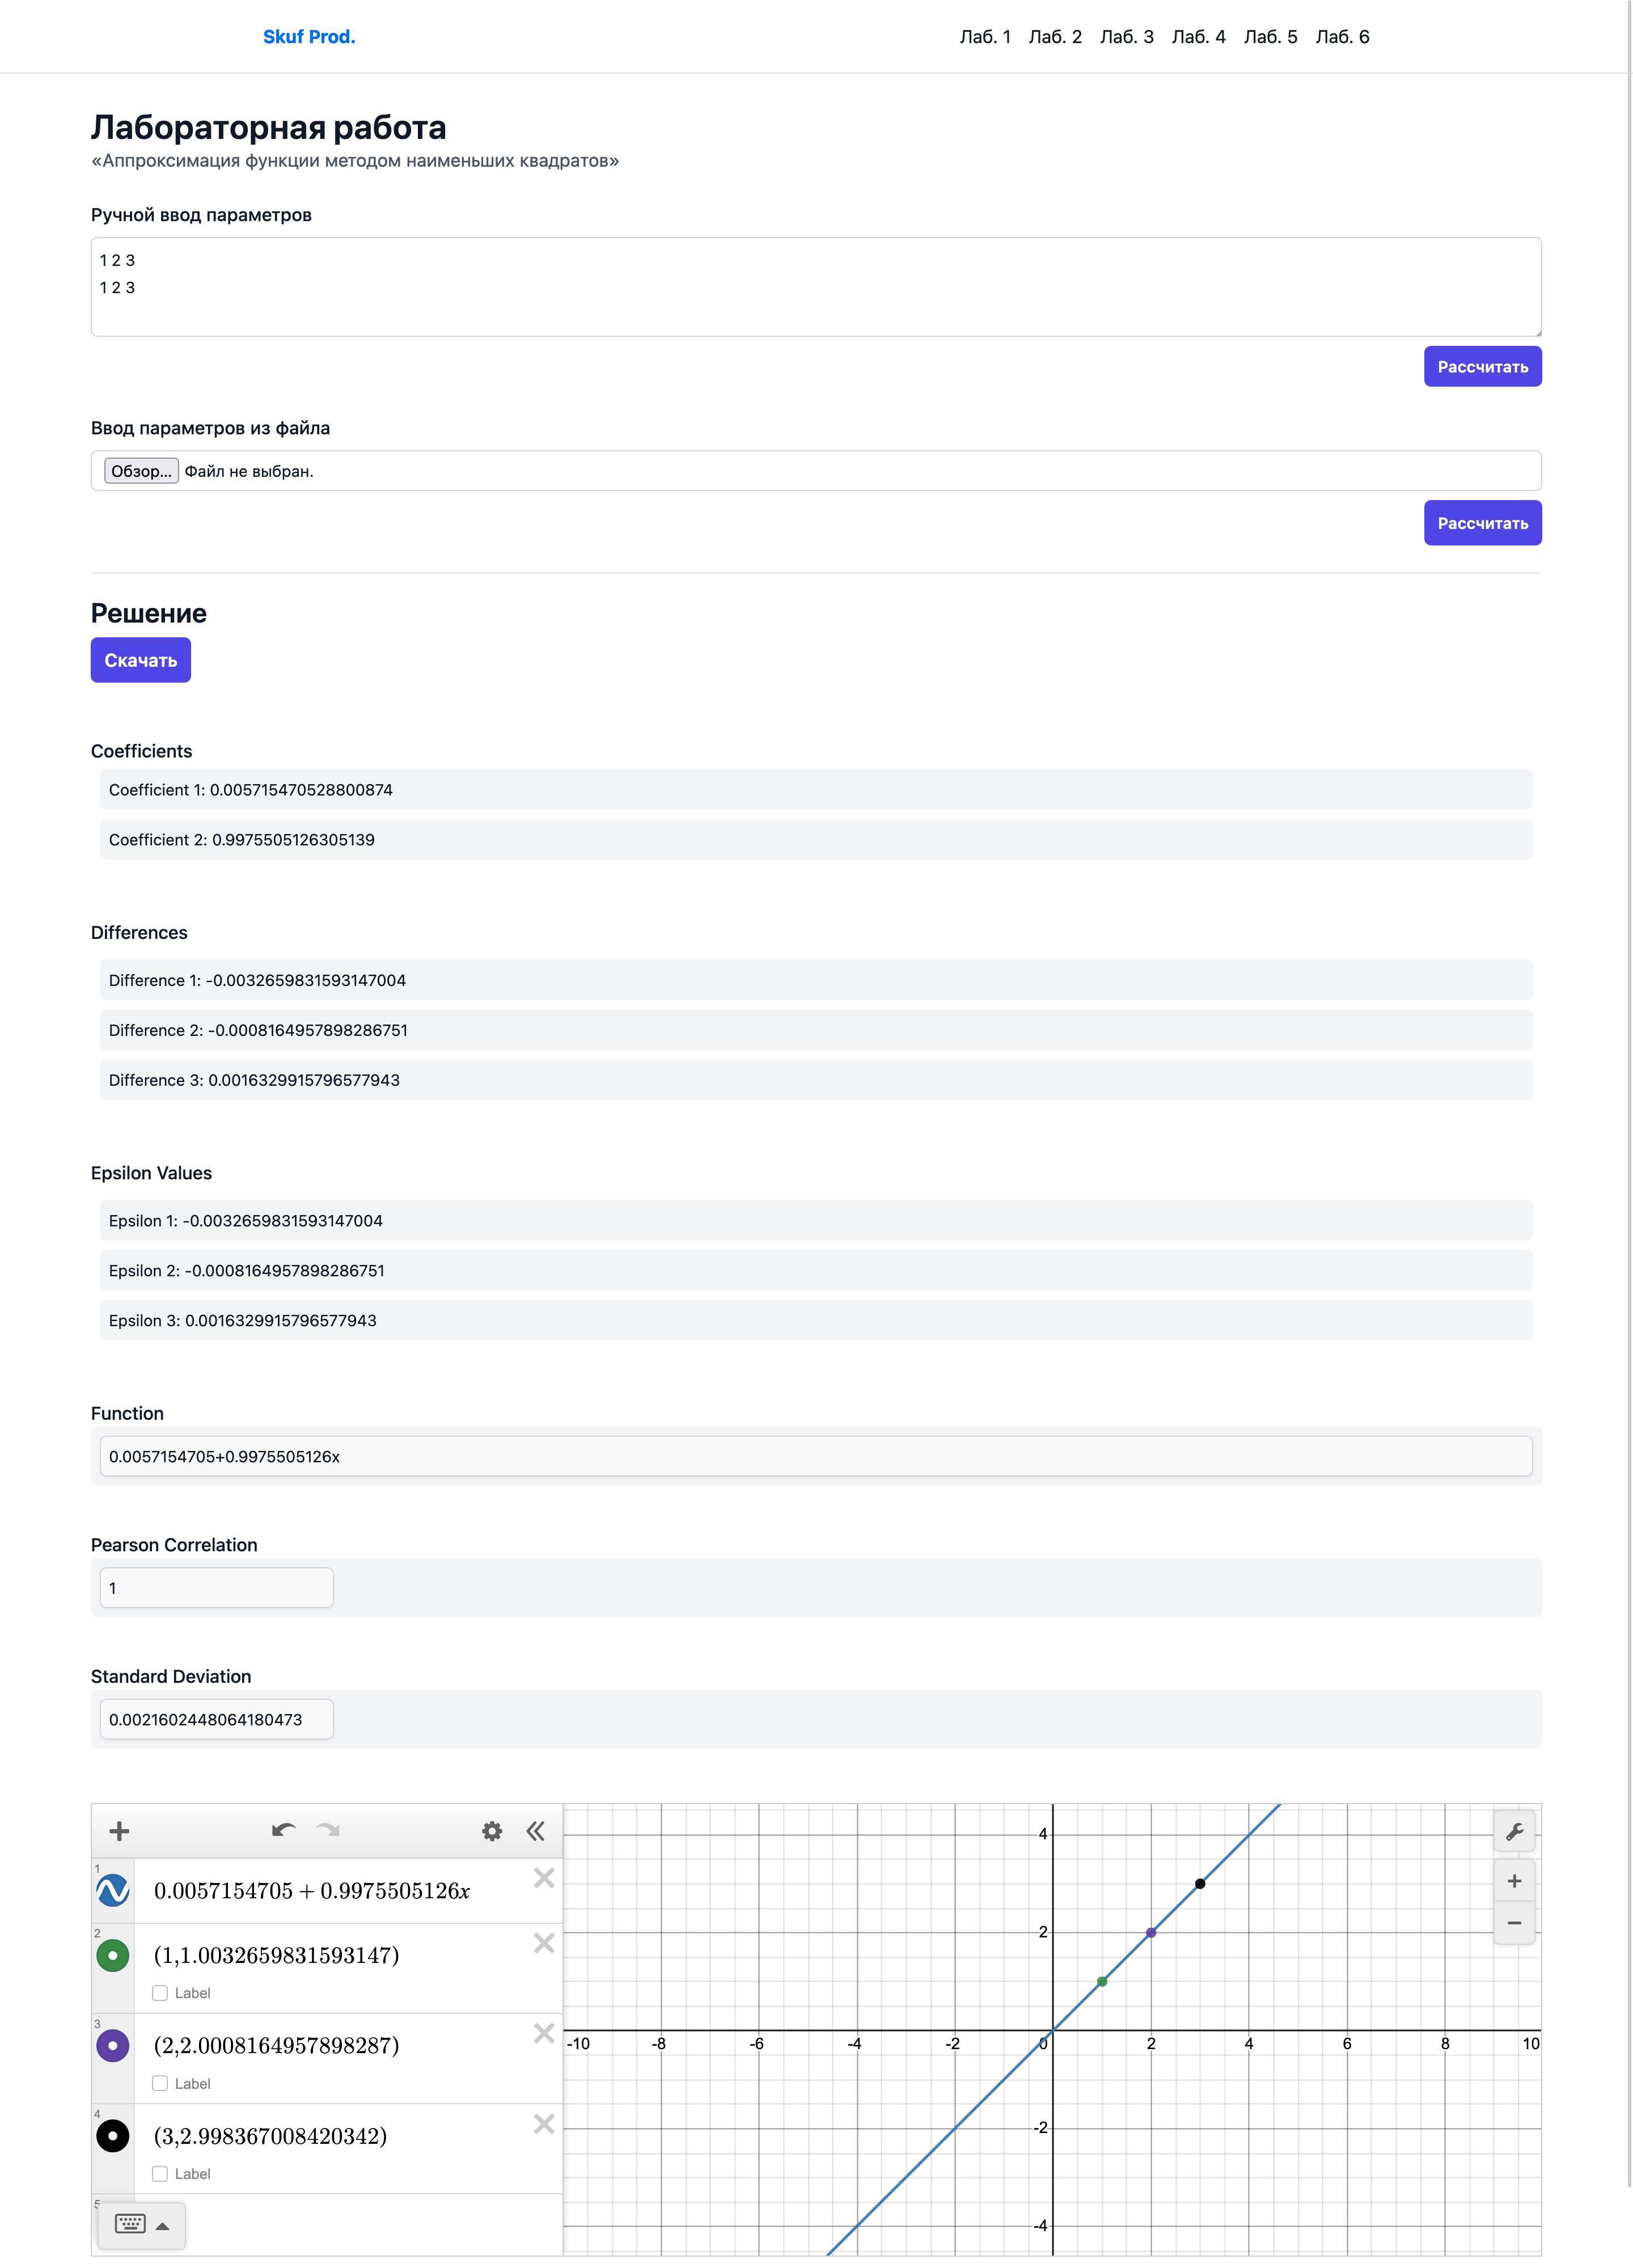
\includegraphics[scale=0.1]{ui.png}
                        \caption{\small \sl {UI  1}}  
                  \end{center}  
            \end{figure}
            
\section{Заключение}
      В ходе выполнения данной ЛР я ознакомился с основыми методами интерполяции. Вообще с кайфом написал программу и посчитал ручками.

\begin{thebibliography}{9}
    \bibitem{Методичка}Слайды с лекций (2023). // Кафедра информатики и вычислительной техники -- Малышева Татьяна Алексеевна, к.т.н., доцент.
\end{thebibliography} 

\end{document}
